\documentclass[12pt, twopage]{article}
\linespread{1.25}

\usepackage[utf8]{inputenc}
\usepackage{amsthm}
\usepackage{amsfonts}
\usepackage[slovak]{babel}
\usepackage{graphicx}
\usepackage[hidelinks, breaklinks]{hyperref}

\theoremstyle{definition}
\newtheorem{example}{Príklad}
\newtheorem{definition}{Definícia}

%[]

\title{\textbf{Funkcie}}
\date{\today}
\author{\textit{Educat - vzdelávacie centrum}}

\begin{document}
	\maketitle
	%\tableofcontents
	
	
	\section{Teória k funkciám}
	\begin{definition}[Funkcia reálnej premennej]
		Funkciou reálnej premennej na množine $A \subseteq \mathbb{R}$ sa nazýva predpis, ktorým je každému prvku množiny A priradené \fbox{práve jedno} reálne číslo, ktoré nazývame \fbox{funkčnou hodnotou}.
	\end{definition}
	
	\begin{definition}[Definičný obor]
		Množina $A \subseteq \mathbb{R}$, ktorej prvkom funkcia priradzuje ich funkčné hodnoty, sa nazýva \fbox{definičný obor} funkcie $f$ a značí sa $D(f)$.
	\end{definition}
	
	\begin{definition}[Obor hodnôt]
		Množina $Y \subseteq R$, ktorej prvky sú priradené funkciou $f$ jej definičnému oboru, sa nazýva \fbox{obor hodnôt} a značí sa $H(f)$.
	\end{definition}
	
	\subsection{Spôsoby určenia funkcie}
	
	Funkciu reálnej premennej vieme graficky zobraziť v pravouhlej sradnicovej sústave. Jednotlivé body $[x, y]$ v rovine pritom spĺňajú podmienku, že $y = f(x)$. Takéto zobrazenie sa potom nazýva \fbox{grafom funkcie $f$}. Samotnú funkciu potom vieme určiť nasledovnými spôsobmi. 
	
	\begin{enumerate}
		\item \fbox{predpisom}, napr. $f: y = 3x - 5$ alebo iný zápis je $f(x) = -6x + 11$
		\item \fbox{vymenovaním svojich prvkov}. Napr. $f = \{[2, 4], [3, 7], [5, 11]\}$. Je to teda množina bodov v rovine.
		\item \fbox{tabuľkou}. Napr.: \\
		\begin{tabular}{|c|c|c|c|c|}
			\hline
			x & 1 & 2 & 3 & 4 \\
			\hline
			y & 2 & 4 & 8 & 16\\
			\hline
		\end{tabular}
		\item \fbox{slovným opisom}. Napr.: Funkcia $f$ priraďuje každému prirodzenému číslu jeho dvojnásobok.
		\item \fbox{grafom}. Napr:\\
		\begin{figure}[h]
			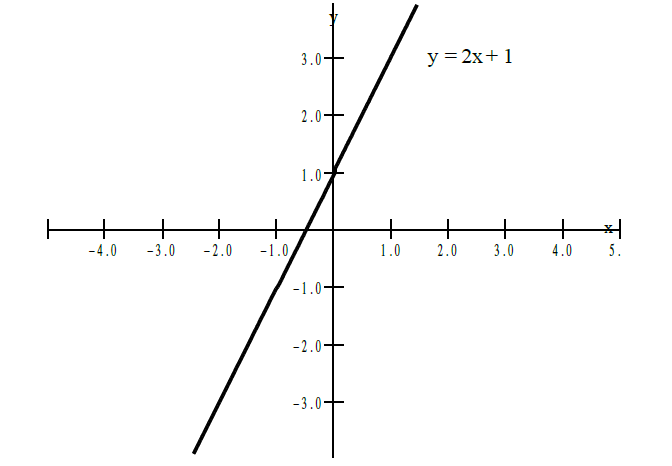
\includegraphics{assets/teoria_graf.png}
		\end{figure}
	\end{enumerate}
	
	\subsection{Vlastnosti funkcií}
	
	\begin{definition}[Párnosť funkcie]
		Funkcia $f$ sa nazýva \fbox{párnou}, ak $\forall x, -x \in D(f): f(x) = f(-x)$.
	\end{definition}
	Graf párnej funkcie je symetrický (dá sa zrkadlovo preklopiť) podľa y-ovej osi.
	
	\begin{definition}[Nepárnosť funkcie]
		Funkcia $f$ sa nazýva \fbox{nepárnou} ak $\forall x, -x \in D(f): f(x) = -f(-x)$.
	\end{definition}
	
	Graf nepárnej funkcie je symetrický podľa počiatku súradnicovej sústavy.
	
	\begin{definition}
		Funkcia $f$ je na množine $M \subseteq D(f)$ \\
		\begin{enumerate}
			\item \fbox{rastúca} ak $\forall x_1, x_2 \in M: x_1 < x_2 \Rightarrow f(x_1) < f(x_2)$
			\item \fbox{klesajúca} ak $\forall x_1, x_2 \in M: x_1 < x_2 \Rightarrow f(x_1) > f(x_2)$
			\item \fbox{neklesajúca} ak $\forall x_1, x_2 \in M: x_1 \le x_2 \Rightarrow f(x_1) \le f(x_2)$
			\item \fbox{nerastúca} ak $\forall x_1, x_2 \in M: x_1 \le x_2 \Rightarrow f(x_1) \le f(x_2)$
		\end{enumerate}
 	\end{definition}
 	
 	Ak je funkcia rastúca/klesajúca/neklesajúca/nerastúca na celom jej definičnom obore, tak skrátene hovoríme, že je rastúca/klesajúca/neklesajúca/nerastúca.
 	
 	\begin{definition}[Monotónnosť]
 		Ak je funkcia na celom definičnom obore iba rastúca, klesajúca, nelesajúca alebo nerastúca, tak ju nazývame \fbox{monotónnou}.
 	\end{definition}
 	
 	\begin{definition}[Rýdza monotónnosť]
 		Ak je funkcia na celom definičnom obore iba rastúca alebo iba klesajúca, tak ju nazývame \fbox{rýdzo monotónnou}.
 	\end{definition}
 	
 	\begin{definition}[Prostosť]
 		Funkcia, sa nazýva \fbox{prostá} ak $\forall x_1, x_2 \in D(f): x_1 \neq x_2 \Rightarrow f(x_1) \neq f(x_2)$.
 	\end{definition}
 	
 	Ak je funkcia rýdzo monotónna, tak je prostá. \textbf{! Naopak ale veta neplatí!}
 	
 	\begin{definition}[Ohraničenosť]
 		Funkcia $f$ sa nazýva \\
 		\begin{enumerate}
 			\item \fbox{zhora ohraničená} ak $\exists h \in \mathbb{R}: \forall y \in H(f) ~ y \le h$
 			\item \fbox{zhora ohraničená} ak $\exists d \in \mathbb{R}: \forall y \in H(f) ~ y \ge d$
 			\item \fbox{ohraničená} ak je ohraničená zdola aj zhora.
 			
 		\end{enumerate}
 	\end{definition}
 	
 	\begin{definition}[Inverzná funkcia]
 		Ak je $f$ prostá funkcia, tak k nej existuje práve jedna funkcia, označme ju $f^{-1}$, ktorá je určená takto:
 		\begin{enumerate}
 			\item jej definičný obor je $H(f)$, teda $D(f^{-1}) = H(f)$,
 			\item $H(f^{-1}) = D(f)$
 		\end{enumerate}
 		Takáto funkcia sa nazýva \fbox{inverznou funkciou} k funkcii $f$.
 	\end{definition}
 	
 	Z týchto dvoch vlastností vyplýva, že graf prostej funkcie je súmerný podľa osi $y = x$ s jej inverziou.
 	
 	\begin{definition}[Periodická funkcia]
 		Funkcia $f$ sa nazýva \fbox{periodická funkcia} práve vtedy, keď existuje $\exists p > 0: \forall k \in \mathbb{Z}:$
 		\begin{enumerate}
 			\item $ak ~ x ~ \in D(f) \Rightarrow x + kp \in D(f)$,
 			\item $f(x + kp) = f(x)$
 		\end{enumerate}
 		Číslo $p$ potom nazývame \fbox{periódou} funkcie $f$.
 	\end{definition}
 	
 	\subsection{Extrémy funkcií}
 	
 	\begin{definition}[Maximum]
 		Hovoríme, že funkcia $f$ má v bode a $\in M \subseteq D(f)$ maximum na množine M práve vtedy, keď pre všetky $x \in M$ platí $f(x) \le f(a)$.
 	\end{definition}
 	
 	\begin{definition}[Minimum]
 		Hovoríme, že funkcia $f$ má v bode a $\in M \subseteq D(f)$ minimum na množine M práve vtedy, keď pre všetky $x \in M$ platí $f(x) \ge f(a)$.
 	\end{definition}
 	
 	\begin{definition}[Ostré maximum]
 		Hovoríme, že funkcia $f$ má v bode a $\in M \subseteq D(f)$ ostré maximum na množine M práve vtedy, keď pre všetky $x \in M$ platí $f(x) \le f(a)$.
 	\end{definition}
 	
 	\begin{definition}[Ostré minimum]
 		Hovoríme, že funkcia $f$ má v bode a $\in M \subseteq D(f)$ ostré minimum na množine M práve vtedy, keď pre všetky $x \in M$ platí $f(x) > f(a)$.
 	\end{definition}
 	
	
	\section{Cvičenia k funkciám}
	
	\url{https://gymmoldava.sk/ICV/CELYWEB/indexICV.php?show=funkcie}
	
	\subsection{Rozhodovačka}
	
	Pre jednotlivé predpisy urči, či predstavujú funkciu, alebo nie.
	\begin{enumerate}
		\item $f = \{ [-1, 2], [0, 0], [1, 2], [2, 3]\}$
		\item $g = \{[-1, 0], [0, -1], [-1, 1], [1, -1]\}$
		\item $h:$
		\begin{tabular}{|c|c|c|c|c|}
			\hline
			x & 1 & 3 & 5 & 7 \\
			\hline
			y & -1 & 2 & 5 & -7 \\
			\hline
		\end{tabular}
		\item $i:$
		\begin{tabular}{|c|c|c|c|c|}
			\hline
			x & -2 & -1 & 0 & 1 \\
			\hline
			y & 1 & 1 & 1 & 2 \\
			\hline
		\end{tabular}
		\item $j:$
		\begin{center}
			\begin{figure}[!htbp]
				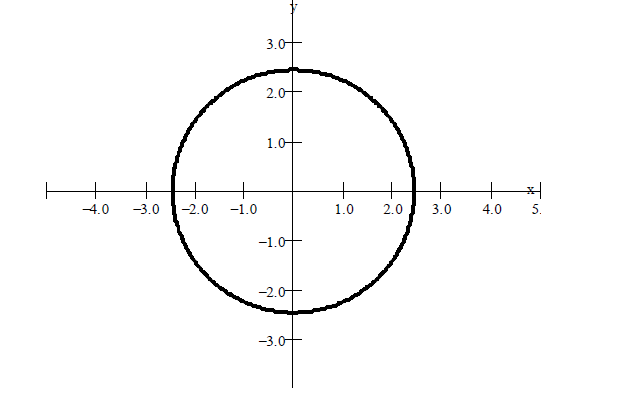
\includegraphics[width=8cm]{assets/jeniejef_kruznica.png}
			\end{figure}
		\end{center}
		
		\item $k:$\\
		\begin{center}
			\begin{figure}[!htbp]
				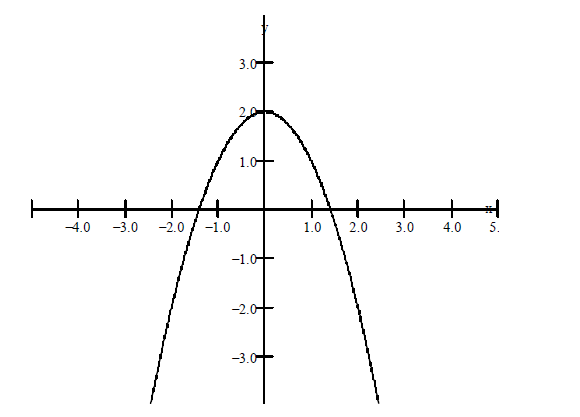
\includegraphics[width=8cm]{assets/jeniejef_parabola.png}
			\end{figure}
		\end{center}


		
	\end{enumerate}
\end{document}